\documentclass[conference]{IEEEtran}
\IEEEoverridecommandlockouts
% The preceding line is only needed to identify funding in the first footnote. If that is unneeded, please comment it out.
\usepackage{cite}
\usepackage{amsmath,amssymb,amsfonts}
\usepackage{algorithmic}
\usepackage{graphicx}
\usepackage{textcomp}
\usepackage{xcolor}
\usepackage[colorlinks = true, urlcolor=blue]{hyperref}
\usepackage{float}
\usepackage{subfig}

\def\BibTeX{{\rm B\kern-.05em{\sc i\kern-.025em b}\kern-.08em
    T\kern-.1667em\lower.7ex\hbox{E}\kern-.125emX}}
\begin{document}

\title{Model Driven Approach for Migration Problem in Hybrid App Development\\}

%TODO: Insert names for each team member%
\author{\IEEEauthorblockN{Zeeshan Khan$^{1}$}
\IEEEauthorblockA{\textit{Faculty of IT} \\
\textit{Monash University}\\
Melbourne, Australia \\
\href{mailto:rqmok@hotmail.com}{rqmok@hotmail.com}}
\and

\IEEEauthorblockN{Mubtasim Mahmud$^{2}$}
\IEEEauthorblockA{\textit{Faculty of IT} \\
\textit{Monash University}\\
Melbourne, Australia \\
\href{mailto:mubtasimmahmud20@gmail.com}{mubtasimmahmud20@gmail.com}}
\and

\IEEEauthorblockN{Riordan Dervin Alfredo$^{3}$}
\IEEEauthorblockA{\textit{Faculty of IT} \\
\textit{Monash University}\\
Melbourne, Australia \\
\href{mailto:riordan.alfredo@gmail.com}{riordan.alfredo@gmail.com}}
\and

\IEEEauthorblockN{Raymond Nguyen$^{4}$}
\IEEEauthorblockA{\textit{Faculty of IT} \\
\textit{Monash University}\\
Melbourne, Australia \\
\href{mailto:rbnguyen1357@yahoo.com.au}{rbnguyen1357@yahoo.com.au}}
\and 

\IEEEauthorblockN{Tomaž Kosar$^{5}$}
\IEEEauthorblockA{\textit{Faculty of Electrical Engineering and Computer Science} \\
\textit{University of Maribor}\\
Maribor, Slovenia \\
\href{mailto:tomaz.kosar@um.si}{tomaz.kosar@um.si}}
}

\maketitle

\begin{abstract}
Software migration is a common problem for developers working in industry or even working on personal projects. It is usually time consuming
and difficult to test if it has been done correctly. Nowadays may web application frameworks have different versions which makes it difficult
to migrate given how frequently they change. One key example is the Ionic Framework which is used to help build desktop as well as mobile applications,
with a simple "write once, deploy anywhere" type of strategy. The Ionic Framework has a manual migration guide that can help developers migrate from 
different versions. We believe that the tedious work involved can be mitigated partially through automation. Therefore we propose a 
model-driven apporach to aid the migration process. By focusing on a model-driven approach, we can develop a model
which is a representation of the system which will generate code for a specific version. Our approach was applied to a case study in order to validate
whether this approach was successful or not. 
\end{abstract}

\section{Introduction}
At some point in the software lifecycle, the current system must be migrated into a new system or version. 
Software migration is the intricate process of moving an application from one environment or version to another. 
Software migration in general, usually consumes lots of resources, time, and effort. 
\\ According to the online article (IBM, 2014) \cite{b1}, it described several common challenges in migrating software applications. In terms of business aspects, these include: determining when to migrate, resistance of users culture and the migration itself not being completed on time. 
For the technical aspects, these include: minimizing disruption of mission critical applications and ensuring that the application functions correctly after migration.
\\ These migration challenges are common for new technologies, especially for web and mobile-based applications as they are constantly changing \cite{b5}. Recently, hybrid apps have become popular as an alternative to native mobile applications due to its overall benefits \cite{b2}. Hybrid applications host a web application inside a 
native webview while utilizing bridges that allow access to native app functions such as camera access, geolocation, etc. 
This means that developers are able to carry over their expertise with web technologies to mobile app development without needing to learn native tech stacks. 
\\ A key example of this is the Ionic Framework which is a very popular hybrid application development framework that employs a ‘write once and run anywhere’ \cite{b3} approach. The latest version of Ionic (version 4) was 
a complete rewrite that makes it incompatible with projects written in Ionic 3, which makes it a suitable candidate for the research project.
\\ There are several differences between Ionic 3 and 4, which makes it worth the port, including compatibility with any front-end framework as opposed to Ionic 3’s tight coupling with Angular. 
There are quite a few issues that can deter development teams from doing a manual port to Ionic 4 which includes breaking changes to the library versions used in both framework versions. Despite there being a guide into how to manually migrate from an Ionic 3 project to an Ionic 4 project, 
there are still a vast number of forums dedicated to help solve the manual migration process. 
\\ One potential solution to solve these problems is to create models to help generate code to support the migration process. 
This might be achieved with a software engineering technique called model-driven development \cite{b4}. Model-driven approaches are used mainly in software design to generally 
simplify a complex process of the system into a higher-level abstraction. By abstracting the migration process into a code generation tool, it could possibly speed up the 
migration process with high accuracy and consistency as intended. In addition, it would benefit developers as it is a more efficient way to deal with the migration problems.
\\ Finally, applying a model driven approach would not just be applicable to the Ionic framework, but potentially other web frameworks as well. 
Therefore, model-driven approaches might solve software migration problems towards hybrid app development in regards to technical and business aspects 
that industry is currently facing. Using a model-driven approach as well as focusing on Ionic versions 3 and 4, the research undertaken will determine whether 
the issue of model driven approaches for migration can be applied. 
\\ This report will go into detail about our research questions and then move into how we approached the problem. Afterwards, we will evaluate our research, looking specifically
at our case study (Meetup For Pets) and other Ionic version 3 projects. Futhermore, the model will be discussed in detail as well as the code generated using this model. Subsequently,  we will discuss our
experiences applying a model-driven approach to solve the migration issue and tie in some other related literature to our own work. Eventually, we will formulate a conclusion and mention possible
future work that our research may have. 
\newline \newline The contributions of this work are as follows:
\begin{itemize}
    \item We will introduce a case study Ionic 3 application (MeetUp For Pets) built primarily to test the viability of a proposed model
    \item A metamodel will be built as well as a model which performs code generation to convert from Ionic 3 to Ionic 4
    \item Our findings and evaluations will then be presented on the feasibility of using a model driven approach for migrating using the Ionic Framework as the primary focus
\end{itemize}

\section{Research Question}
Looking into the problem a bit more, we have devised a main research question below.
\newline \newline \textbf{Can model-driven development provide a valid migration solution?}
\newline \newline Branching away from this primary question, we have additional research questions that target the concerns about the migration tool we are proposing:
\begin{enumerate}
    \item RQ: Can it account for major changes like different libraries/versions?
    \newline Looking at the Ionic Framework, there are specific libraries or versions used in a project that may differ from one version to another. 
    These may involve small changes like simply changing the name to match the new version or larger changes such as changing the way the application handles routing to different pages. 
    Our research will involve taking a look at some of these changes.
    \item RQ: Is generated code of acceptable quality?
    \newline With the model being used to help convert one Ionic 3 project file to a compatible Ionic 4 version, there can be a chance that the migration may not be perfect. 
    There might be flaws with the output of the conversion which breaks the integrity of the original file. Our research will also observe the quality of the code and take note of any changes.
    \item RQ: Can the tool be used for other case studies?
    \newline Our modelling tool will be primarily used for our case study (Meetup For Pets) however every Ionic project is expected to be different. 
    Our research will observe to see if the tool will be applicable not just for our case study, but for other Ionic 3 projects as well. 
\end{enumerate}

\section{Approach}
\subsection{The Modelling Tool}

In order to migrate the case study application from one version to another, the migration tool was modelled. This section describes how the Eclipse Modeling Framework and Acceleo has been used for this purpose.

\subsubsection{Eclipse Modeling Framework}

The Eclipse Modeling Framework (EMF), is a standard for data models with full support for meta-modelling and modelling \cite{b11}.

During this research, EMF has been used to create a meta-model from which a model for the migration tool has been derived. EMF is pre-configured with the Ecore meta-metamodel (or super-metamodel) for constructing the domain-specific meta-model.

\subsubsection{Overview of Operation}

After creating the metamodel and, hence, the model, Acceleo has been utilised to help call the appropriate operations in the model to read the source files, modify its contents, and then write back to the files. Figure \ref{fig:operation} shows a diagram of this workflow.

\begin{figure}[htbp]
\centerline{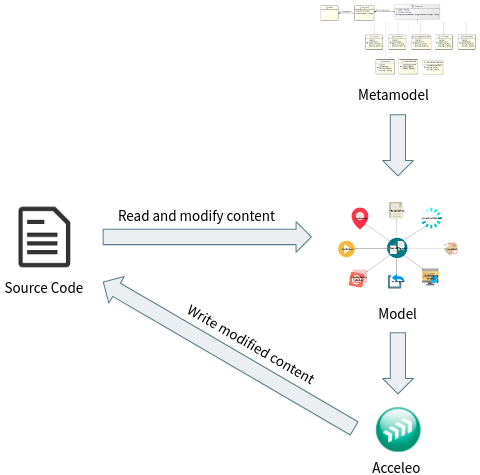
\includegraphics[width=\linewidth,keepaspectratio]{workflow.png}}
\caption{Migration Tool Operation Overview}
\label{fig:operation}
\end{figure}

\subsubsection{The Metamodel}

The solution to the migration tool metamodel is shown in Figure \ref{fig:metamodel}. The metamodel contains an entity called \textit{mBase}, which is used as a container for all other entities for creating the model.

\begin{figure}[htbp]
\centerline{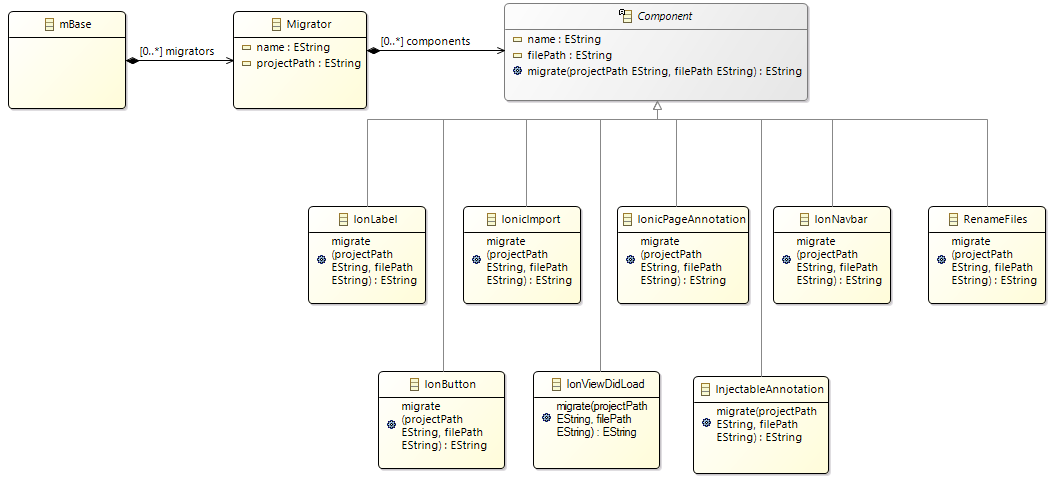
\includegraphics[width=\linewidth,keepaspectratio]{metamodel.png}}
\caption{Migration Tool Metamodel}
\label{fig:metamodel}
\end{figure}

The \textit{Migrator} entity stores the path to the project that needs to be migrated. It contains a set of \textit{Components}. Each \textit{Component} entity is a part of the source code for the application that needs to be migrated.

Each \textit{Component} contains a path to the file, relative to the project path, that contains the source code for that component, and also a \textit{migrate} operation. The \textit{migrate} operation is given the project path and the file path relative to the project path. The operation combines these paths to produce an absolute path and read the file to modify its contents.

These components are separated in the metamodel rather than the model because each one has a separate way of migrating the source code that it is responsible for. Furthermore, each of the \textit{migrate} operations for the components are manually written in Java and inserted into the Java source files generated by EMF.

\subsubsection{The Model}

Once the metamodel Java source code is generated and the \textit{migrate} operation for each \textit{Component} is manually inserted into this code, the migration tool can finally be modelled.

\begin{figure}[htbp]
\centerline{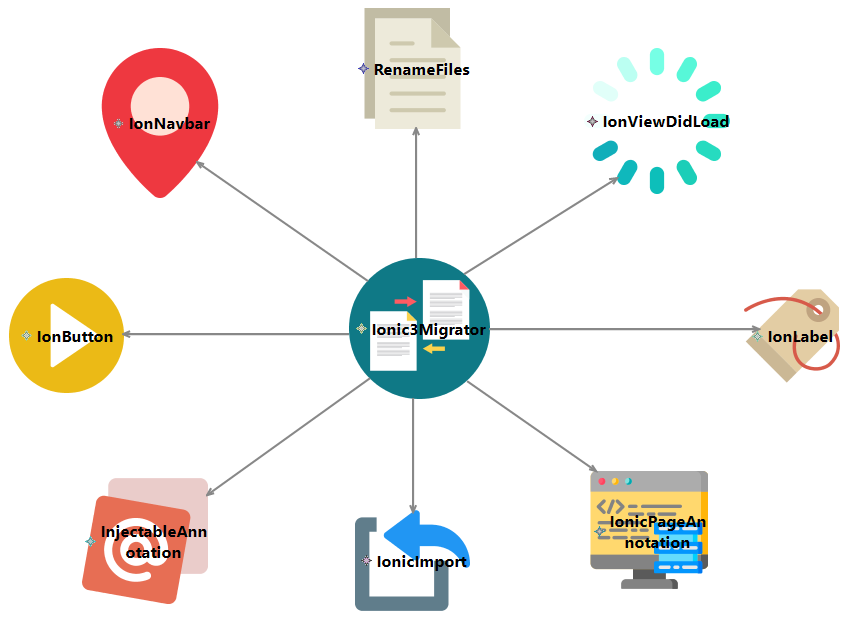
\includegraphics[width=\linewidth,height=\textheight,keepaspectratio]{model.png}}
\caption{Migration Tool Model}
\label{fig:model}
\end{figure}

Figure \ref{fig:model} shows the migration tool’s model, which simply contains instances of the entities that were created in the metamodel. Through this model, the project path is provided to the \textit{Migrator} entity instance, and the individual file paths relative to the project path are provided to each \textit{Component} entity instance.

Sirius is an Eclipse project that allows for creating a graphical modelling workbench in EMF \cite{b12}. It has been used to visualise the model shown in Figure \ref{fig:model}.

\subsubsection{Acceleo}

Acceleo is a template-based source code generation technology to facilitate model-to-text transformations (MTT). It is used as an add-on for EMF to be used with the model \cite{b13}.

The model in Figure \ref{fig:model} contains a project path, file path for each \textit{Component}, and a \textit{migrate} operation in each component that takes both paths as its parameters. In order to utilise these operations, Acceleo is used as shown in Figure \ref{fig:acceleo}.

\begin{figure}[htbp]
\centerline{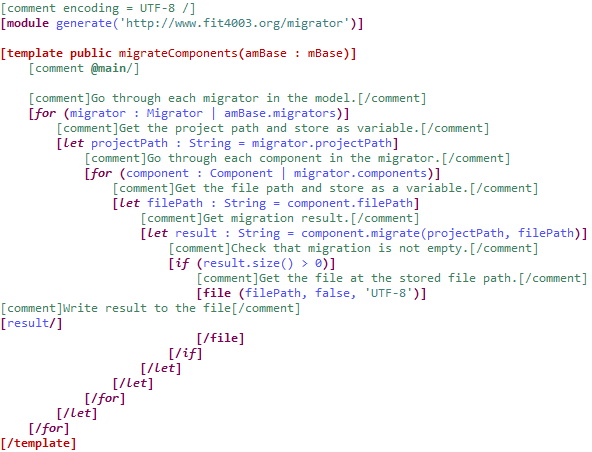
\includegraphics[width=\linewidth,keepaspectratio]{acceleo.png}}
\caption{Migration Tool Acceleo Script}
\label{fig:acceleo}
\end{figure}

The Acceleo script in Figure \ref{fig:acceleo} goes through each migrator’s components in the model, retrieves the project path and file path from a component, and calls that component’s \textit{migrate} operation, giving it both paths as parameters. The \textit{migrate} operation then returns a string that contains the contents of the entire file including the migration modifications. Acceleo will then write this string back to the file, essentially overwriting the entire file. However, the script ignores writing to a file when the \textit{migrate} operation returns an empty string. This can be useful for operations that do not require changing a file’s contents.

\subsubsection{Running the Migration Tool}

Once the model is created, and the project path and file path are given, the Acceleo script is run by creating the appropriate run configuration in EMF.

The model gives flexibility to the user by allowing a \textit{Component} to be removed if it shouldn’t be included in the migration process, and then added back in if it does. However, it should be remembered that the file path will always need to be given where the component resides in the source code, and each file will need to have a separate \textit{Component} created for it.

\section{Evaluation}

\subsection{Case Study}
As a proof-of-concept, the application that will be developed for our case study will be called \textbf{Meetups for Pets}. It is a hybrid application written 
in Ionic version 3 to connect pet enthusiasts to promote face-to-face interactions with pets and their owners. The users will have the ability to organise a 
meetups with each pet’s owner. The main purpose of this case study is to test the model-driven migration tool, this can be shown in Figure \ref{fig:meetupIonic}
\begin{figure}%
    \centering
    \subfloat[The home page of Meetup for Pets]{{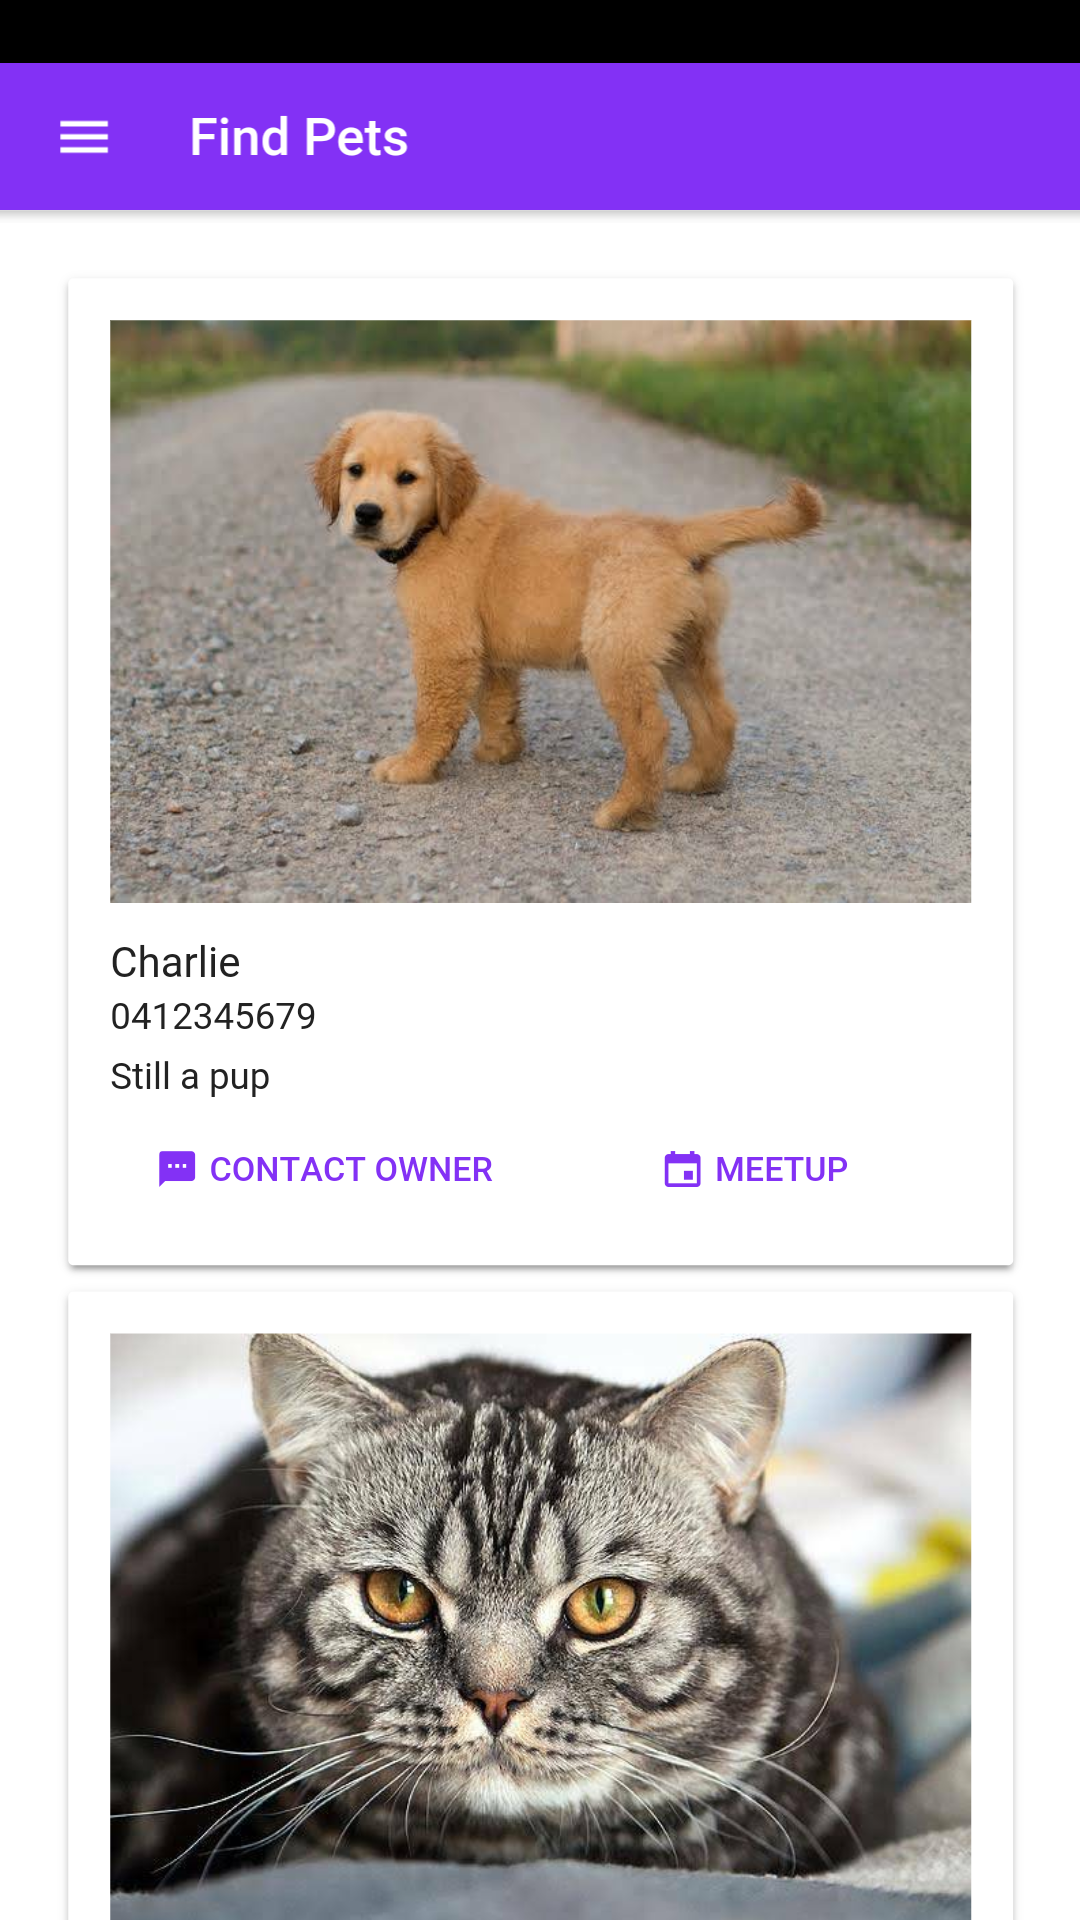
\includegraphics[scale=0.1]{find_pets.png} }}%
    \qquad
    \subfloat[A list of pets that a user owns]{{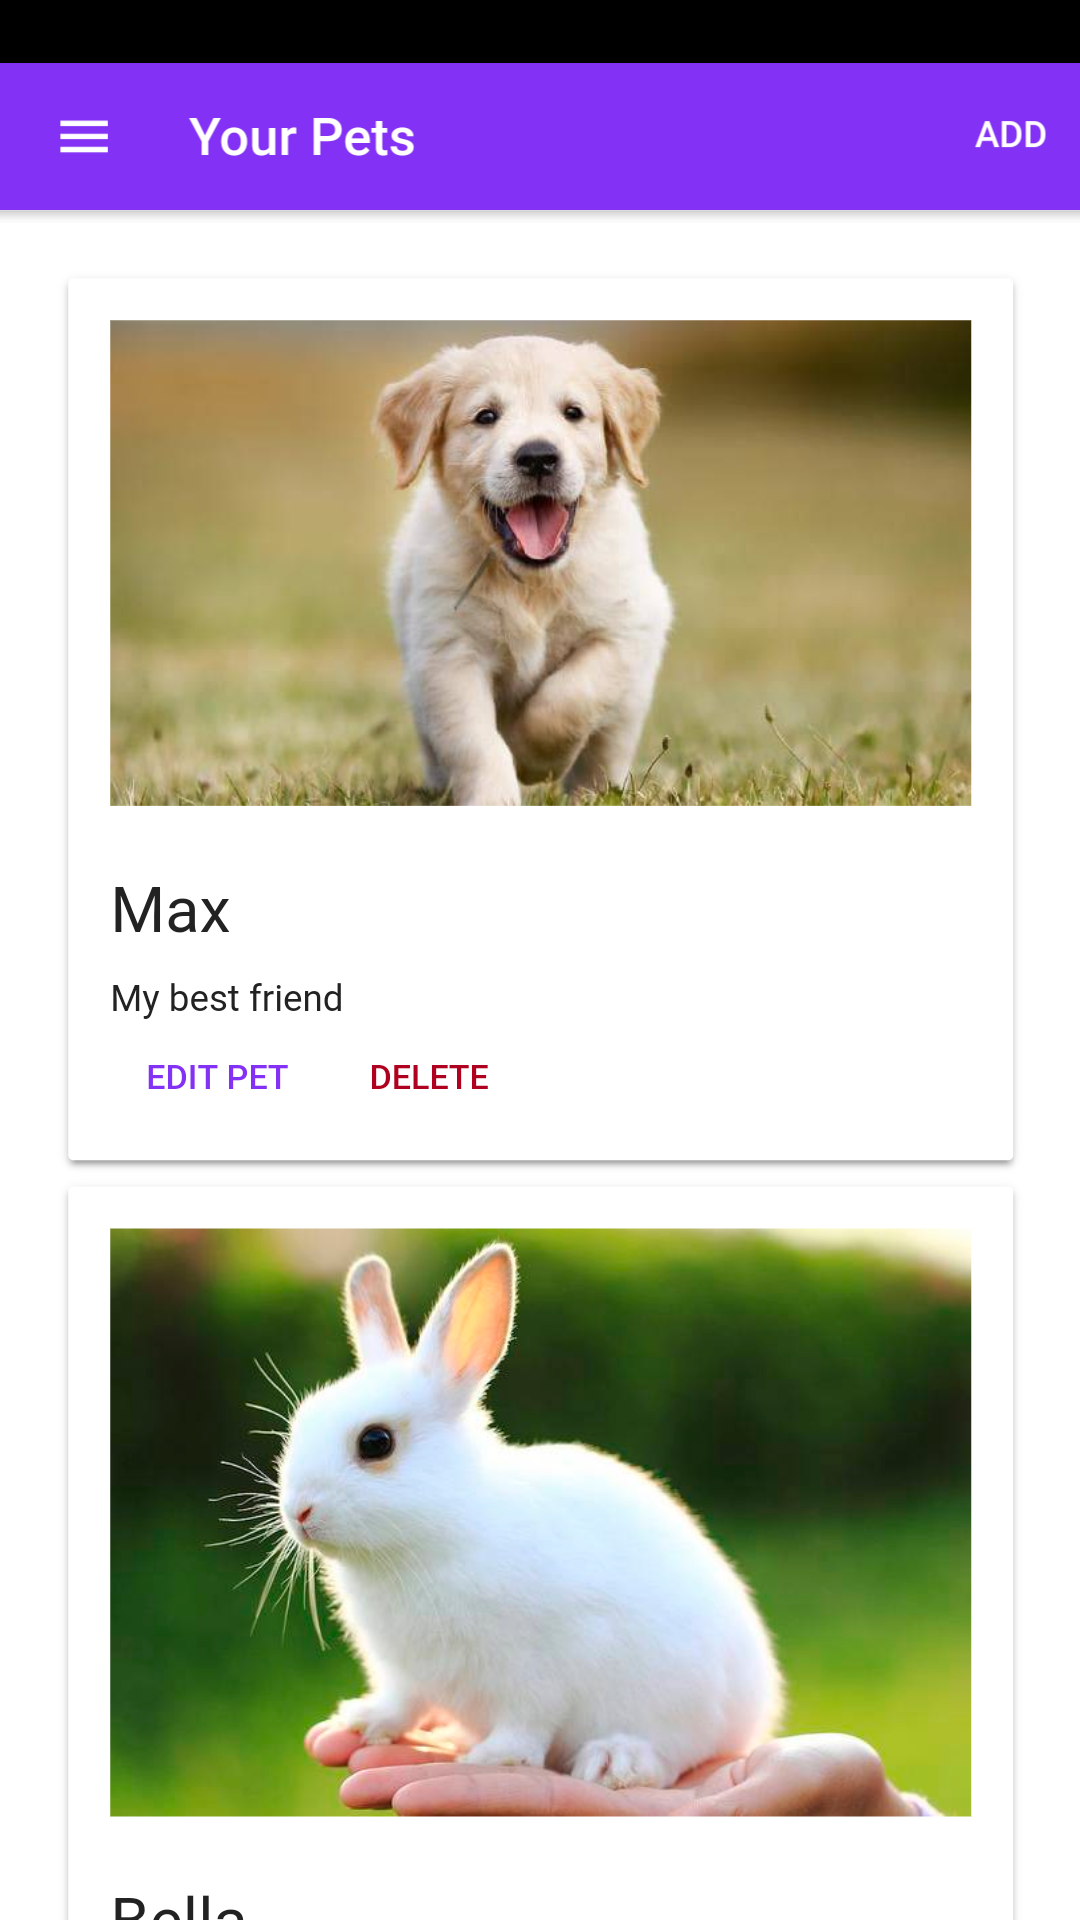
\includegraphics[scale=0.1]{your_pets.png} }}%
    \caption{Meetup For Pets Ionic 3 Application}%
    \label{fig:meetupIonic}%
\end{figure}
\\ In a real-world scenario, an application would normally take advantage of the hardware capabilities of the device it is running on. 
Therefore, there are some Ionic native framework features that were included, such as camera, contacts, calendar, and messaging.
\\ Using the case study above, we attempted to perform some manual migration to look deeper into the issues that may arise when migrating. In our research we had also attempted to use another open-source Ionic 3 application from GitHub \cite{b14} in order to test if our model 
had generated the correct Ionic 4 code.

\subsection{The Model}


\subsection{Code Generation}
The results of the migration tool we developed were quite favorable. The case study
involved migrating three categories of changes:
\begin{enumerate}
    \item HTML markup
    \item Typescript code
    \item Architectural changes (file and folder structure)
\end{enumerate}

\subsubsection{HTML Markup}
The migration tool tackles the problem by separating the full
text into components (.i.e buttons, labels, etc.). This is the most
general category, as the migration process for different components
has a lot of common procedures.
\begin{figure}[!htb]
    \centering
    \subfloat[Ionic 3]{
        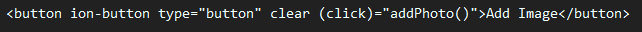
\includegraphics[width=0.8\linewidth]{button.PNG}
        \label{fig:ion3button}
    }
    \qquad
    \subfloat[Ionic 4]{
        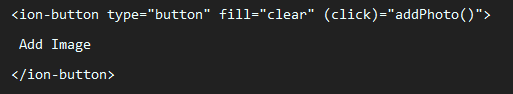
\includegraphics[width=0.8\linewidth]{buttonv4.PNG}
        \label{fig:ion4button}
    }
    \caption{Ionic 3-4 Button Migration (Markup)}
    \label{fig:ionicButtonMigration}
\end{figure}

\subsubsection{Typescript code}
Migration of Typescript code involves looking through code files
to find specific tokens and changing them to fit the Ionic 4 specification.
Unlike HTML markup, every different migration process in this category is almost
completely different, and can only be generalized in broad terms, such as find-and-replace
functionality.
\begin{figure}[!htb]
    \centering
    \subfloat[Ionic 3]{
        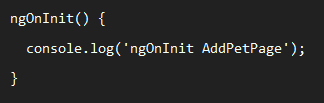
\includegraphics[width=0.8\linewidth]{lifecycle.PNG}
        \label{fig:lifecycle3}
    }
    \qquad
    \subfloat[Ionic 4]{
        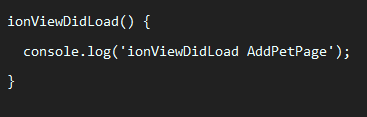
\includegraphics[width=0.8\linewidth]{lifecyclev4.PNG}
        \label{fig:lifecycle4}
    }
    \caption{Ionic 3-4 Lifecycle Methods Migration (Typescript)}
    \label{fig:ionicLifecycleMigration}
\end{figure}

\subsubsection{Architectural Changes}
The structure of an Ionic 4 project is drastically different from an Ionic 3 project,
making its migration a very specific process. The tool focuses on a small subset, which
involves reorganizing files associated with one specific feature of an app to the equivalent Ionic 4
folder structure, as well as renaming them to fit the new convention.
\begin{figure}[!htb]
    \centering
    \subfloat[Ionic Feature Migration Output]{
        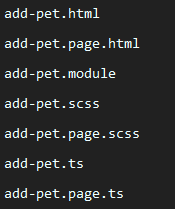
\includegraphics[width=0.8\linewidth]{files.PNG}
        \label{fig:ionFiles}
    }
    \caption{Ionic 3-4 File Rename-and-Relocate Migration (Architectural)}
    \label{fig:ionicFileMigration}
\end{figure}


\section{Discussion/Experiences}
The overall consensus is that model-driven development is a feasible approach
for software migration, especially regarding this case study in particular.
\newline \newline
For HTML markup in particular, automating component-wise migration is remarkably simple, and it
is well within the scope of possibility to create a general function that will migrate any Ionic
3 component to its Ionic 4 equivalent, provided a library of changes specific to each component
is collated for use by this function.
\newline \newline
Typescript code can be a little more complicated to deal with. During development of the tool,
we encountered some difficulty with porting over two components in particular - \textbf{Toasts} and
\textbf{Alerts}. The difficulty stems from the asynchronous nature of the two in Ionic 4 as opposed to their
counterparts in Ionic 3 - handler function callbacks and deeply nested toasts and alerts have to be handled differently,
which makes migrating these a more involved process than just pure automation.
\newline \newline
Architectural changes vary in difficulty. A project-wide relocation and renaming of files is well within the
scope of possibility, but changes to the routing mechanisms adopted in the different versions are drastic and
require significant changes to the codebase. Ionic 4 uses the routing functionality provided by the frontend framework
specified when creating a project using its command-line interface, meaning that a separate migration process would need
to be adopted for, say, React vs. Angular, for example. Ionic 3 used its own proprietary router on the other hand, which means
at least that part of the code is easier to deal with. While Ionic 4 adopted this change in order to be future-proof, this does
make a generalized migration tool for this specific feature a lot harder to implement.

% @Author: Riordan Dervin Alfredo, 2/11/2019 %
\section{Related Work}
In regards to the software migration that utilises model driven engineering methods,
there are already several studies that were conducted extensively before.
Those are; Migrating C/C++ Software to Mobile Platforms in the ADM Context \cite{b6},
FASMM: Fast and Accessible Software Migration Method \cite{b7}, Reverse Engineering 
Strategies for Software Migration \cite{b8}, Model-Driven Engineering 
for Software Migration in a Large Industrial Context \cite{b9}, and
Towards a Model-Driven Approach for Planning a 
Standard-Based Migration of Enterprise Applications to SOA \cite{b10}
\newline \newline
According to Martinez et al.\cite{b6} study is related to our work in terms of processing different kinds of 
programming languages and paradigms to generate mobile application code. It is also 
the main feasible example of a model-driven approach in the software migration of native-mobile applications,
which is in our case is the migration of the hybrid mobile application.
This study took an example of C/C++ language to produce Android, iOS, and Windows mobile applications. 
In our study, the extension type of the generated code is still maintained, but the main code-generation process with this study 
is technically similar. 
\newline \newline
Furthermore, this study gives insight in regards to the feasibility of a model-driven development approach that is 
advanced to ADM (Architecture-Driven Modernization) within a similar domain, mobile application migration. 
The validation tool that is used in this study is the same as what we are using in our approach, which is the Eclipse Modelling Framework \cite{b2}.
Mobile applications are formed using different kinds of programming languages, which is technically 
how hybrid application systems work.
The ADM approach that is described in this study could potentially be part of our future works. 
\newline \newline
In terms of methodologies, our study is closely related to the FASMM approach as described by Forite, et al. \cite{b3} .
This study provides extensive guides and methods to conduct software migration. The migration
process that it is aiming is at the short and non-optimised migration phase.
It is frequently quickly done and not necessarily in an optimized way. For example,
inaccurate functionalities implementation, loose new architecture, and non-capitalised gained knowledge
during the migration. These conditions are relatable with the environemnt of our current study.
Therefore, our study followed the described methodologies that enables validation of 
hybrid application migration process with model-driven engineering techniques. It also allows
capitalising knowledge as transformation rules, to make it highly reusable in the future migration projects.
\newline \newline

In \cite{b9} and \cite{b10} studies are proving the feasibility of model-driven engineering
in different domains and contexts from our studies. Those are the migration to a completely new framework, 
migration to a new architecture (legacy achitecture to service-oriented architecture), and migration
of different languages to specific mobile application framework. 
They also provided insights on how model-driven engineering processes are economically
profitable and are cost-effective. 
\newline \newline
In the paper \cite{b9}, author describes the process of migrating a large-scale software application from Mainframe to J2EE
using Model-Driven Engineering process. The migration process in this study starts by describing the general 
processes of the current legacy system.
First, a parser is created to make an abstract syntax tree from the legacy code. Then, it is processed
by a transformation to build a model that conforms to the meta-model of the legacy language.
During the second stage, all symbols are resolved and bound to the appropriate model elements.
Afterwards, from the model representing the code, a reverse-engineering process is conducted to produce a platform independent 
model. Finally, this model will be mapped into a platform specific model that can be used to generate code
for the final product of the migrated application.
\newline \newline
Lastly, Aboulsamh describes \cite{b10} the feasibility of model-driven approaches to be used in the software migration context in general.
Our proposed method that utilises model transformation to generate the migrated code conforms with this 
research arguments. The migration system that it utilises are a sequential execution of model transformation \cite{b10}
that is quite similar to our approach. 
However, this research uses much more complex software migration modelling 
methodologies that is slightly irrelevant with our current study objectives. These are including
the usage of service model and migration path model to defines common meta-data for semantic integration.
\section{Conclusion}
In conclusion, our study contributes to another area in software migration with 
model-driven engineering methodologies, focusing on the hybrid application domain.
At this stage, our approach only proves a small fraction of the hybrid application migration because 
this study only focused on one framework (Ionic) and only based on the selected versions (version 3 to version 4).
\newline \newline
At the moment, within various constraints, the validation tool that we had developed only handles basic migration functionalities.
More specifically it is only using string parsing, transformations, and code-generation. These processes might
be insufficient to handle more complex functionalities as described in our limitations.
\newline \newline
This leads to many other challenges that need to be tackled in the proposed methods to fully migrate the Ionic version 3 project
to version 4. The main goal in this study is to prove the feasibility of migration hybrid application with model-driven engineering
methods, and it is proven to be true. Therefore, building fully-functional software migration tool for hybrid application is intentionally 
left for future work. 
\newline \newline
Here, we used the Eclipse Modeling Framework as validator and main migration tool to handle migration process of 
the Ionic framework from version 3 to version 4. Within this tool, the abstraction level was intentionally 
increased for the cohesiveness and extensibility of migration functions. By following our approaches and methodologies, 
future researchers could add and upgrade the tool to handle more complex functionalities according 
to limitations as described above.
\newline \newline
At the moment, our approaches are only applicable to solve basic software migration problems in hybrid application. 
It requires more extensive researches to solve more complex functionalites, such as dealing with 
architectural changes to arrange files in the correct directories. ADM (Architecture-Driven Modernization) and 
KDM (Knowledge Discovery Metamodel) methods \cite{b6} \cite{b10} could potentially be the candidates to solve 
current limitations in this study. 
\newline \newline
There will be time in the future for this tool to be mature enough so that the migration of Ionic Framework applications 
from version  3 to version 4 can be done thoroughly, without introducing any migration bugs.
This tool is also envisioned to handle migration of Ionic framework from 
any versions to the latest. In the future, by following our approaches and adding on further researches, 
it could potentially migrate the other hybrid application frameworks.

\begin{thebibliography}{00}
\bibitem{b1} "IBM Knowledge Center", Ibm.com, 2019. [Online]. Available: \url{https://www.ibm.com/support/knowledgecenter/en/SSEP7J_10.2.1/com.ibm.swg.ba.cognos.ug_mfdm.10.2.1.doc/c_mfdm_chal_mig.html}. [Accessed: 07-Sep-2019].
\bibitem{b2} B. Dunka, E. Emmanuel and D. Oyeyinka, "Hybrid Mobile Application Based on Ionic Framework Technologies", \textit{International Journal of Recent Advances in Multidisciplinary Research}, Vol. 04, Issue 12, p. 3121-3130, 2017. [Accessed: 27-Aug-2019].
\bibitem{b3} M. Huynh, P. Ghimire and D. Truong, "Hybrid App Approach: Could It Mark The End of Native App Domination?", \textit{Issues Informing Science and Information Technology Education}, Vol. 14, p. 49-65, Hammond, LA, 2017. [Accessed: 07-Sep-2019].
\bibitem{b4} García Díaz, Vicente \& Núñez Valdez, Edward \& Espada, Jordán  \& Pelayo García-Bustelo, B. \& Cueva Lovelle, Juan \& Marín, Carlos, "A brief introduction to model-driven engineering", Vol. 18, p. 127-142, 2014. [Accessed: 27-Aug-2019].
\bibitem{b5} J. Kwon and S. Moon, "Web Application Migration with Closure Reconstruction", \textit{International World Wide Web Conference Committee (IW3C2)}, Seoul, 2014. [Accessed: 23-Aug-2019].
% Related works' biblioraphies %
\bibitem{b6} Martinez, L., Pereira, C., Favre, L., ``Migrating C/C++ Software to Mobile Platforms in the ADM context,'' \textit{International Journal of Interactive Multimedia and Artificial Intelligence}, Vol. 4 , N\textsuperscript{o}3, p. 34, 2017. [Abstract].
\bibitem{b7} Forite, L. and C. Hug. ``FASMM: Fast and Accessible Software Migration Method,'' in Research Challenges in Information Science (RCIS), 2014 IEEE Eights Internation Conference on. 2014, IEEE.
\bibitem{b8} Muller, H. A. ``Reverse Engineering Strategies for Software Migration'', in Proceedings of the (19\textsuperscript{th}) International Conference on Software Engineering, May 1997, p. 659, IEEE.
\bibitem{b9} Fleurey, F., Breton, E., Baudry, B., Nicolas, A., Jezequel, J., ``Model-Driven Engineering for Software Migration in a Large Industrial Context'', in International Conference on Model Driven Engineering Languages and Systems, 2007, pp. 482-497, MODELS
\bibitem{b10} Aboulsamh, M.A. ``Towards a Model-Driven Approach for Planning a Standard-Based Migration of Enterprise Applications to SOA'', in 2009 Congress on Services - l , 2009, IEEE.
\bibitem{b11} R. Gronback, "Eclipse Modeling Project | The Eclipse Foundation", Eclipse.org, 2019. [Online]. Available: \url{https://www.eclipse.org/modeling/emf/}. [Accessed: 04- Nov- 2019].
\bibitem{b12} "Sirius - Overview", Eclipse.org, 2019. [Online]. Available: \url{https://www.eclipse.org/sirius/overview.html}. [Accessed: 04- Nov- 2019].
\bibitem{b13} "Acceleo | Home", Eclipse.org, 2019. [Online]. Available: \url{https://www.eclipse.org/acceleo/}. [Accessed: 04- Nov- 2019].
\bibitem{b14} "growu/drip-ionic3", GitHub, 2019. [Online]. Available: https://github.com/growu/drip-ionic3, 2019 [Accessed: 14-Oct-2019].
\end{thebibliography}
\vspace{12pt}
\color{red}

\end{document}
